\chapter{Theoretical Background}

\section{Reinforcement Learning}

By definition, Reinforcement Learning (RL) algorithms learn solutions for sequential decision processes via 
repeated interaction with an environment \cite{albrecht2024multi}. An agent simply refers 
to a decision maker that receives information from the environment and takes actions based
on that. The environment is defined as the external system with which the agent interacts, 
and may change state according to some transition dynamics, giving the agent a feedback (or reward).
The agent's goal is to learn an optimal decision making policy that let him obtain 
the maximum cumulative reward over time. This optimal policy is obtained by trying 
different actions in different states and observing the outcomes, in a trial-and-error fashion.

Moreover, RL differs from other machine learning paradigms, like supervised or unsupervised learning, 
in that it does not require labeled input-output pairs, and the rewards act as a proxy from which to learn 
an optimal policy.

\subsection{Markov Decision Process}

Going into a more mathematical and formal definition, a sequential decision process 
can be modeled as a Markov Decision Process (MDP), which consists of:
\begin{itemize}
    \item A set of states $S$;
    \item A set of actions $A$;
    \item A reward function $R : S\times A\times S \to \mathbb{R}$;
    \item A state transition probability function $P : S\times A\times S \to [0,1]$ such that in state $s$ taking action $a$ the probability of transitioning to state $s'$ is $p(s'|s,a)$;
    \item A policy $\pi : S \to A$ that maps states to actions, such that in state $s$ the agent takes action $a$ with probability $\pi(a|s)$;
    \item A discount factor $\gamma \in [0,1]$ that determines the importance of future rewards.
\end{itemize}

An MDP starts in an initial state $s_0$, sampled from the initial state distribution. At each time step $t$, the agent 
observes the current state $s_t$, takes an action $a_t$ according to its policy $\pi(a_t|s_t)$ and receives a reward 
$r_t = R(s_t, a_t, s_{t+1})$, where $s_{t+1}$ is the next state sampled from the transition probability distribution $p(s_{t+1}|s_t, a_t)$.
Once the terminal state is reached, or after the maximum number of time steps, the episode ends. Figure~\ref{fig:1} shows the described framework.

\begin{figure}
    \centering
    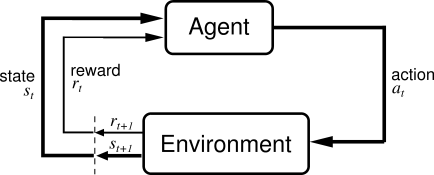
\includegraphics[width=0.6\textwidth]{assets/agent-env.png}
    \caption{MDP framework.}
    \label{fig:1}
\end{figure}

\subsection{Value function}

The Markov property states that the future state $s_{t+1}$ depends only on the current state $s_t$ and action $a_t$, 
and not on the previous states and actions.

\begin{equation}
    Pr(s_{t+1},r_t|s_t,a_t,s_{t-1},a_{t-1},...,s_0,a_0) = Pr(s_{t+1},r_t|s_t,a_t)
\end{equation}

Therefore, in an MDP, the expected return can be defined individually for each state $s \in S$, creating the concept of \textit{value function}. 

\begin{align}
    V_{\pi}(s) &= \mathbb{E}_{\pi}\left[r_t + \gamma r_{t+1} + \gamma^2 r_{t+2} + \dots | s_t = s\right] \\
    &= \sum_{a \in A}\pi(a|s) \sum_{s' \in S} \mathcal{P}(s'|s,a)\left[\mathcal{R}(s,a,s') + \gamma\mathbb{E}_{\pi}\left[u_{t+1}|s_{t+1}=s'\right]\right] \\
    &= \sum_{a \in A}\pi(a|s) \sum_{s' \in S} \mathcal{P}(s'|s,a)\left[\mathcal{R}(s,a,s') + \gamma V_{\pi}(s')\right]
\end{align}

This is referred to as the Bellman equation, and it defines a system of $m$ linear equations with $m$ variables ($m=|S|$) and a unique solution, given by the value function $V_{\pi}$ for policy $\pi$.
If all elements of the MDP are known, the value function can be computed by solving the system of equations. However, in most real-world scenarios, the transition probabilities and reward functions are unknown, and the agent must learn the value function through interaction with the environment.

\subsection{PPO}
Value-based RL methods are a class of RL algorithms that learn a value function, which is used to estimate the expected return of a state or state-action pair. The value function is usually represented as a neural network with parameters $\theta$, and it is updated using the Bellman equation. The value function can be used to derive a policy by selecting the action that maximizes the expected return.
The loss function is usually defined as squared error between the value function estimate and the target value $y_t$:
\begin{equation}
    \mathcal{L}(\theta) = \left(y_t - \mathcal{Q}(s_t,a_t;\theta)\right)
\end{equation}
where $y_t$ is the target value, defined as:
\begin{equation}
    y_t = \begin{cases}
        r_t + \gamma \max_{a'}\mathcal{Q}(s_{t+1},a_{t+1};\theta) & \text{if } s_{t+1} \text{ is not terminal} \\
        r_t & \text{if } s_{t+1} \text{ is terminal}
    \end{cases}
\end{equation}

Since the loss function contains the approximate value function twice, and we want to update the value estimate for the current state-action pair,
the solution is to stop any gradient flow backward through the target, to avoid computing gradients through the bootstrapped target value. In fact, 
the bootstrapped value estimate should only serve as a target value to optimize the main value estimate $\mathcal{Q}(s_t,a_t;\theta)$ toward.

To reduce the instability of training caused by the bootstrapped target value,
the target network is used, which is a different neural network with parameters $\phi$ that is used to compute bootstrapped target values.
Its parameters are periodically updated by copying the current parameters of the main value function network to the target network.
Another problem is the correlation of consecutive experiences. The update of value function parameters with most recent experiences may lead 
to the agent forgetting optimal policies learned in the past and in other experiences. This is due to the fact the changes in the policy will lead to 
changes in the data distribution encountered by the agent, which then lead to changes in the optimal policy. The usual solution is to randomize the experience samples used to train the agent,
that is why the replay buffer is used. In fact, a batch of experiences is sampled uniformly at random from the replay buffer, which will be used to 
update the value function parameters. This way, experiences can be reused multiple times (which leads to more efficient sampling) and gradients are more stable and with lower variance.

Policy gradient methods, instead, are a class of RL algorithms that learn a parameterized policy directly, without the need for a value function. The policy is usually represented as a neural network with parameters $\phi$, and it is updated using the policy gradient theorem. 
It provides a theoretically founded expression for the gradient of the performance of a parameterized policy with respect to the parameters of the policy.
\begin{equation}
    \nabla_{\phi}J(\phi) \propto \sum_{s\in \mathcal{S}}Pr(s|\pi)\sum_{a\in\mathcal{A}}Q^{\pi}(s,a)\nabla_{\phi}\pi(a|s;\phi)
\end{equation}

where $J$ represents a function measuring the quality of a policy $\pi$. It is similar to a loss function, but it is maximized and not minimized.
\begin{align}
    J(\phi) &= \mathbf{E}_{\pi}\left[\sum_{k}\gamma^k r_{t+k}\right] \\
            &= \sum_s Pr(s'|s,a)\sum_a\pi(a|s;\phi)\left[R_t+\gamma V_{\pi}(s_{t+1})\right]
\end{align}

Then, by writing the policy gradient as an expectation with respect to the probability of states occurring under the current policy and the probability of actions being selected by the policy:
\begin{equation}
    \nabla_{\phi}J(\phi) = \mathbf{E}_{s\sim Pr(\cdot|\pi),a\sim\pi(\cdot|s)}\left[Q^{\pi}(s,a)\nabla_{\phi}\log\pi(a|s;\phi)\right]
\end{equation}
This illustrates how the optimization of the parameterized policy is limited to on-policy only data.

The expectation in the policy gradient can be either approximated or obtained from samples. REINFORCE uses Monte Carlo estimation as a sampling method, which uses on-policy samples of episodic returns to approximate the expected returns of the policy.
It minimizes the following loss function:
\begin{equation}
    \mathcal{L}(\phi) = -\frac{1}{T}\sum_{t=0}^{T-1}\left(\sum_{\tau=t}^{T-1}\gamma^{\tau-t}r^{\tau}\right)\log \pi(a^t|s^t;\phi)
\end{equation}
Each episode, a full trajectory is collected by using current policy $\pi$, and then the return estimate is computed to estimate the policy gradient. 
However, Monte Carlo return estimates come with high variance and unstable training. Usually, the subtraction of a baseline (which keeps the bias but reduces the variance) is used as a solution.

Actor-critic algorithms train a parameterized policy (the actor) and a value function (the critic), alongside each other. The actor is optimized using gradient 
estimates derived from the policy gradient theorem, while the critic is used to compute bootstrapped return estimates. These estimates allow to estimate episodic 
returns just from the experience of a single step:
\begin{equation}
    \mathbf{E}_{s^t\sim Pr(\cdot|\pi)}\left[u(h^t)|s^t\right] = \mathbf{E}_{s^t\sim Pr(\cdot|\pi),a^t\sim\pi(\cdot|s^t),s^{t+1}\sim \mathcal{T}(\cdot|s^t,a^t)}\left[\mathcal{R}(s^t,a^t,s^{t+1}) + \gamma V(s^{t+1})|s^t\right]
\end{equation}
Moreover, bootstrapped return estimates exhibit lower variance compared to the Monte Carlo estimates of episodic returns, with the cost of introduced bias, since the value function might not approximate the true expected returns of states.
Essentially, a trade-off between bias and variance has to be made, and intermediate solutions are available just by estimating $N$-step returns, aggregating the received rewards of $N$ consecutive steps before computing a value estimate of the last state.

Advantages of the current policy can be computed to guide the policy gradients:
\begin{equation}
    Adv^{\pi}(s,a) = Q^{\pi}(s,a) - V^{\pi}(s)
\end{equation}
An advantage represents how much better or worse an action is compared to the average action in a given state. 
For a positive value, then, the probability of the policy $\pi$ choosing that action should be increased, while for a negative value it should be decreased. The advantage function can be estimated using the critic's value function as:
\begin{equation}
    Adv(s^t,a^t) = Q(s^t,a^t) - V(s^t) = \begin{cases} r^t + V(s^t) \quad \text{if }s^{t+1}\text{ is terminal} \\
    r^t + \gamma V(s^{t+1}) - V(s^t) \quad \text{otherwise}
    \end{cases}
\end{equation} 

Therefore, the actor loss to be minimized becomes:
\begin{equation}
    \mathcal{L}(\phi) = -Adv(s^t,a^t)\log\pi(a^t|s^t;\phi)
\end{equation}

And the critic loss is defined as:
\begin{equation}
    \mathcal{L}(\theta) = (y^t - V(s^t;\theta))^2
\end{equation}

Furthermore, entropy regularization can be added to the actor loss to discourage premature convergence to a suboptimal policy and incentivize exploration. 
It is a measure of the policy's uncertainty, and minimizing the negative entropy penalizes it for assigning a very high probability to any action.
\begin{equation}
    -\mathcal{H}(\pi(\cdot|s;\phi)) = \sum_{a\in\mathcal{A}}\pi(a|s;\phi)\log\pi(a|s;\phi)
\end{equation}

Since the individual gradient update steps could lead to large policy updates, the idea of Trust Regions was introduced in TRPO \cite{schulman2015trpo}, which 
essentially constrain the policy updates to a small area within the space of policy parameters in which the policy would not change significantly. 
PPO, instead, computes a computationally efficient surrogate objective to avoid large jumps in policy optimization steps. It makes use of importance sampling weights $\rho(s,a)$, which are defined
as the fraction of probabilities of selecting a given action $a$ in a state $s$ for two policies:
\begin{equation}
    \rho(s,a) = \frac{\pi(a|s;\phi)}{\pi_{\beta}(a|s)}
\end{equation}
This factor adjusts the data distribution to make the data generated by $\pi_{\beta}$ appear on-policy for $\pi$. Using these weights, PPO is able to update the policy multiple times using the same data and restrict the change of the policy by restricting the importance sampling weight.
In fact, the actor loss becomes:
\begin{equation}
    \mathcal{L}(\phi) = -\min \left(\rho(s^t,a^t)Adv(s^t,a^t), \text{clip}(\rho(s^t,a^t),1-\epsilon,1+\epsilon)Adv(s^t,a^t)\right)
\end{equation}

Algorithm~\ref{alg:ppo} summarize the whole procedure.

\begin{algorithm}[t]
\caption{PPO}
\label{alg:ppo}
\begin{algorithmic}[1]
\State Initialize actor network $\pi$ with random parameters $\phi$
\State Initialize critic network $V$ with random parameters $\theta$
\State Repeat for every episode:
\For{time step $t = 0,1,2,\dots$}
    \State Observe current state $s^t$
    \State Sample action $a^t \sim \pi(\cdot|s^t;\phi)$
    \State Apply action $a^t$; observe reward $r^t$ and next state $s^{t+1}$
    \State $\pi_{\beta}(a^t|s^t) \gets \pi(a^t|s^t;\phi)$ \Comment{store the old policy probability}
    \For{epoch $e=1,\dots,N_e$}
        \State $\rho(s^t,a^t) \gets \frac{\pi(a^t|s^t;\phi)}{\pi_{\beta}(a^t|s^t)}$
        \If{$s^{t+1}$ is terminal}
            \State Advantage $Adv(s^t,a^t)\gets r^t - V(s^t;\theta)$
            \State Critic target $y^t \gets r^t$
        \Else
            \State Advantage $Adv(s^t,a^t)\gets r^t + \gamma V(s^{t+1};\theta) - V(s^t;\theta)$
            \State Critic target $y^t \gets r^t + \gamma V(s^{t+1};\theta)$
        \EndIf
        \State Actor loss $\mathcal{L}(\phi)\gets -\min \left(\rho(s^t,a^t)Adv(s^t,a^t), \text{clip}(\rho(s^t,a^t),1-\epsilon,1+\epsilon)Adv(s^t,a^t)\right)$
        \State Critic loss $\mathcal{L}(\theta)\gets (y^t - V(s^t;\theta))^2$
        \State Update parameters $\phi$ by minimizing the actor loss $\mathcal{L}(\phi)$
        \State Update parameters $\theta$ by minimizing the critic loss $\mathcal{L}(\theta)$
    \EndFor
\EndFor
\end{algorithmic}
\end{algorithm}

\section{Multi-agent Reinforcement Learning}

When multiple agents are taken into consideration, the concept of Multi-agent Reinforcement Learning (MARL)
comes into play. In MARL, multiple agents interact with the same environment at the same time, and their 
actions can affect each other's rewards and state transitions. Moreover, each agent has its own long-term reward
to optimize, which now becomes a function of the policies of all other agents \cite{zhang2021multi}. 

\subsection{Markov Games}

Markov Games (MGs) are a generalization of MDPs to the multi-agent setting, and are defined by a tuple ($\mathcal{N}, \mathcal{S}, \left\{\mathcal{A}^i\right\}_{i\in\mathcal{N}}, \mathcal{P}, \left\{\mathcal{R}^i\right\}_{i\in\mathcal{N}}, \gamma$), where $\mathcal{N} = \left\{1,\dots,N\right\}$ denotes the set of agents, $\mathcal{S}$ denotes the state space observed by all agents, $\mathcal{A}^i$ denotes the action space of agent $i$.
Let $A:=A^1\times\dots\times A^N$ denote the joint action space, then $\mathcal{P}:\mathcal{S}\times \mathcal{A}\to\delta(\mathcal{S})$ denotes the transition probability function from any state $s\in\mathcal{S}$ to any state $s'\in\mathcal{S}$ for any joint action $a\in\mathcal{A}$; $R^i:\mathcal{S}\times\mathcal{A}\times\mathcal{S}\to\mathbb{R}$ is the reward function that determines the immediate reward received by agent $i$ for a transition from ($s,a$) to $s'$; $\gamma \in [0,1)$ is the discount factor.

At each time step $t$, each agent executes an action $a^i_t$ according to the system state $s_t$. The system transitions to a new state $s_{t+1}$ and gives each agent a reward $r^i_t$. Each agent wants to maximize its long-term reward, finding a policy $\pi^i$. As a consequence, the value-function $V^i : \mathcal{S}\to\mathbb{R}$ of agent $i$ becomes a function of the joint policy $\pi$ defined as $\pi(a|s) = \prod_{i\in\mathcal{N}}\pi^i(a^i|s)$.

\begin{equation}
    V^i_{\pi^i,\pi^{-i}} := \mathbb{E}\left[\sum_{t\geq 0}\gamma^t R^i(s_t,a_t,s_{t+1}) | a^i_t \sim \pi^i(\cdot | s_t), s_0 = s\right]
\end{equation}

Since each agent's value function depends on the policies of all other agents, the optimal policy for each agent is defined as a Nash equilibrium, where no agent can improve its long-term reward by unilaterally changing its policy.
A Nash equilibrium is a joint policy $\pi^* = (\pi^{1*},\dots,\pi^{N*})$ such that for all agents $i\in\mathcal{N}$ and for all states $s\in\mathcal{S}$, we have:

\begin{equation}
    V^i_{\pi^{i,*},\pi^{-i,*}}(s) \geq V^i_{\pi^i,\pi^{-i,*}}(s), \quad \forall \pi^i
\end{equation}

In other words, at a Nash equilibrium, each agent's policy is the best response to the policies of all other agents, and no agent can improve its long-term reward by changing its policy while the others keep theirs fixed.
It always exists for finite-space infinite-horizon discounted MGs, but may not be unique in general.

\subsection{Cooperative setting}

In some tasks, agent may need to cooperate to achieve a common goal, and in these cases they share a common reward function, i.e., $R^1 = R^2 = \dots = R^N = R$. 
With this model in mind, the value function and Q-function are identical to all agents, which thus enables the single-agent RL algorithms to be applied, if all agents are coordinated as one decision maker. 
Moreover, agents are allowed to have different reward functions, which may be kept private to each agent, while the goal for cooperation is to optimize the long-term reward corresponding to the average reward $\bar{R}(s,a,s') := N^{-1}\cdot\sum_{i\in\mathcal{N}}R^i(s,a,s')$ for any $(s,a,s')\in\mathcal{S}\times\mathcal{A}\times\mathcal{A}$. 

\subsection{Challenges of MARL}

MARL algorithms may be useful in many real-world applications, but they face several challenges that make them more difficult to design and analyze than single-agent RL algorithms.

\begin{itemize}
    \item \textbf{Non-stationarity}: since multiple agents learn concurrently, the environment faced by each agent is non-stationary, since the action taken by one agent affects the reward of other opponent agents, and the evolution of the state. As a result, each agent needs to learn to account for how other agents behave and adapt to the joint behavior accordingly. In fact, if each agent ignores this issue and optimizes its own policy assuming a stationary environment (\textit{independent learning}), the algorithms may fail to converge. 
    \item \textbf{Non-unique learning goals}: the learning goals in multi-agent settings may be unclear or conflicting, as each agent may have its own objectives and preferences, which may not align with those of other agents. This can lead to situations where agents are competing for resources or trying to achieve different goals, making it difficult to design algorithms that can effectively balance the needs of all agents.
    \item \textbf{Credit assignment problem}: in multi-agent settings, it can be difficult to determine which agent's actions contributed to the overall outcome, especially when the agents are working together towards a common goal. This can make it challenging to assign credit or blame for the success or failure of the team, and can lead to suboptimal learning outcomes.
    \item \textbf{Scalability}: to handle non-stationarity, each individual agent may need to account for the joint action space, whose dimension increases exponentially with the number of agents. This can make it difficult to scale MARL algorithms to large numbers of agents, as the computational and communication requirements may become prohibitive.
    \item \textbf{Partial observability}: in many real-world scenarios, agents may not have access to the full state of the environment, and may only be able to observe a limited subset of the state variables. This can make it difficult for agents to learn effective policies, as they may not have enough information to make informed decisions.
\end{itemize}